\documentclass[nobib]{tufte-handout}

\title{Lecture 4: Spectral graph theory and the matrix-tree theorem $\cdot$ 1MA020}

\author[Vilhelm Agdur]{Vilhelm Agdur\thanks{\href{mailto:vilhelm.agdur@math.uu.se}{\nolinkurl{vilhelm.agdur@math.uu.se}}}}

\date{3 November 2023}


%\geometry{showframe} % display margins for debugging page layout

\usepackage{graphicx} % allow embedded images
  \setkeys{Gin}{width=\linewidth,totalheight=\textheight,keepaspectratio}
  \graphicspath{{graphics/}} % set of paths to search for images
\usepackage{amsmath}  % extended mathematics
\usepackage{booktabs} % book-quality tables
\usepackage{units}    % non-stacked fractions and better unit spacing
\usepackage{multicol} % multiple column layout facilities
\usepackage{lipsum}   % filler text
\usepackage{fancyvrb} % extended verbatim environments
  \fvset{fontsize=\normalsize}% default font size for fancy-verbatim environments

\usepackage{color,soul} % Highlights for text

% Standardize command font styles and environments
\newcommand{\doccmd}[1]{\texttt{\textbackslash#1}}% command name -- adds backslash automatically
\newcommand{\docopt}[1]{\ensuremath{\langle}\textrm{\textit{#1}}\ensuremath{\rangle}}% optional command argument
\newcommand{\docarg}[1]{\textrm{\textit{#1}}}% (required) command argument
\newcommand{\docenv}[1]{\textsf{#1}}% environment name
\newcommand{\docpkg}[1]{\texttt{#1}}% package name
\newcommand{\doccls}[1]{\texttt{#1}}% document class name
\newcommand{\docclsopt}[1]{\texttt{#1}}% document class option name
\newenvironment{docspec}{\begin{quote}\noindent}{\end{quote}}% command specification environment

\include{mathcommands.extratex}

\begin{document}

\maketitle% this prints the handout title, author, and date

\begin{abstract}
\noindent
We introduce the basic notions of spectral graph theory, such as the adjacency and incidence matrices of a graph. We build up the theory around these, eventually arriving at the Kirchhoff matrix-tree theorem, which will let us count spanning trees in a graph.
\end{abstract}

Throughout this lecture, we will assume that $G = (V, E)$ is a graph on $n$ vertices, with vertex set $[n]$, and $m$ edges $\{e_1, \ldots, e_m\}$.

\begin{definition}
    The \emph{adjacency matrix} $A$ of a graph $G$ is the $n\times n$ matrix having entries $A_{ij} = 1$ if $i$ and $j$ are neighbours, and zero otherwise.
\end{definition}

\begin{figure}
    \centering
    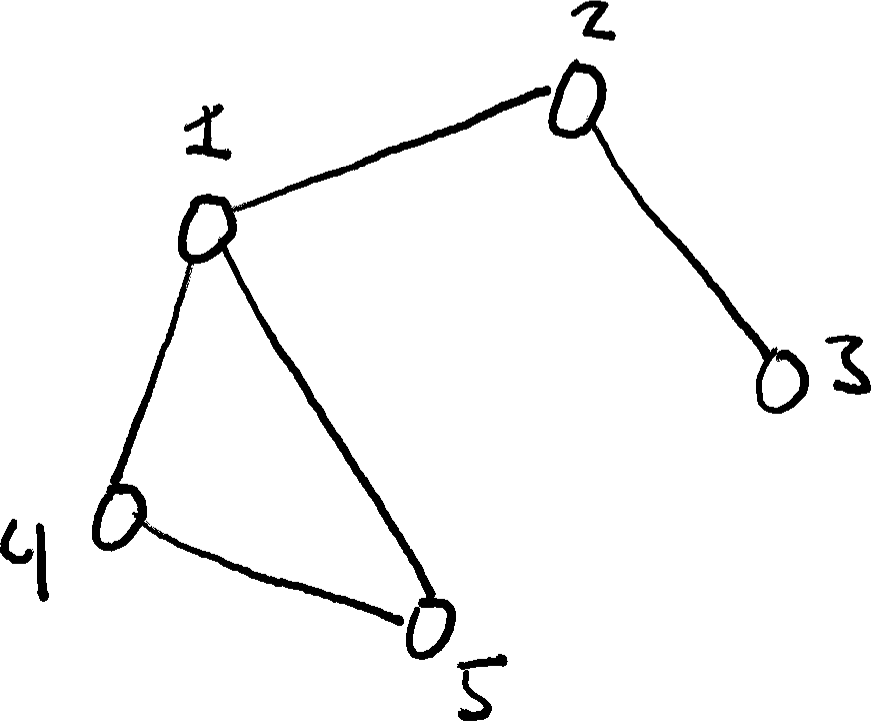
\includegraphics[width=0.3\textwidth]{graphics/L4_spectral/graph_for_adjmat.png}
    \caption{A graph whose adjacency matrix we compute in an example.}
    \label{fig:graph_for_adjmat}
\end{figure}

\begin{example}
    The graph given in Figure \ref{fig:graph_for_adjmat} has adjacency matrix
    $$\begin{pmatrix}
        0 & 1 & 0 & 1 & 0 \\
        1 & 0 & 1 & 0 & 0 \\
        0 & 1 & 0 & 0 & 0 \\
        1 & 0 & 0 & 0 & 1 \\
        0 & 0 & 0 & 1 & 0 
        \end{pmatrix}.$$
\end{example}

\begin{remark}
    There are a few things we can notice immediately about adjacency matrices. First off, they must be symmetric, since of course $i$ and $j$ being neighbours is the same statement as $j$ and $i$ being neighbours, and the diagonal entries are always zero. Second, the row sums or the column sums give us the degree of each vertex, since a row contains one $1$ per edge incident to its vertex.

    Finally, it follows from the spectral theorem for symmetric matrices that all eigenvalues of $A$ are real.
\end{remark}

There is another way to turn a graph into a matrix that is very useful, but it is easiest to define it first for directed graphs, so we begin by giving a definition of a directed graph.

\begin{definition}
    A \emph{directed graph} $G = (V,E)$ (or \emph{digraph} for short) consists of a set of vertices $V$ and a set of edges $E$, where each edge is a tuple of two distinct\sidenote[][]{It is entirely possible to define what we mean by a directed multigraph as well, but for our purposes, we stick to simple directed graphs with no loops or parallel edges.} vertices. We call the first vertex in the tuple the \emph{source} and the second vertex the \emph{target} of the edge.
\end{definition}

Having said this, we can now define the incidence matrix of a directed graph.

\begin{definition}
    The \emph{incidence matrix} $D$ of a digraph $G$ is the $n\times m$ matrix having entries $D_{ij}$, where
    \begin{equation*}
        D_{ij} = \begin{cases}
            1 &\text{if } i \text{ is the target of } e_j\\
            -1 &\text{if } i \text{ is the source of } e_j\\
            0 &\text{otherwise.}
        \end{cases}
    \end{equation*}

    For a simple graph $G$ and a matrix $D$, we say that $D$ is \emph{an} incidence matrix of $G$ if there is a way to direct the edges of $G$ so that the incidence matrix of this directed version is $D$.
\end{definition}

\begin{figure}
    \centering
    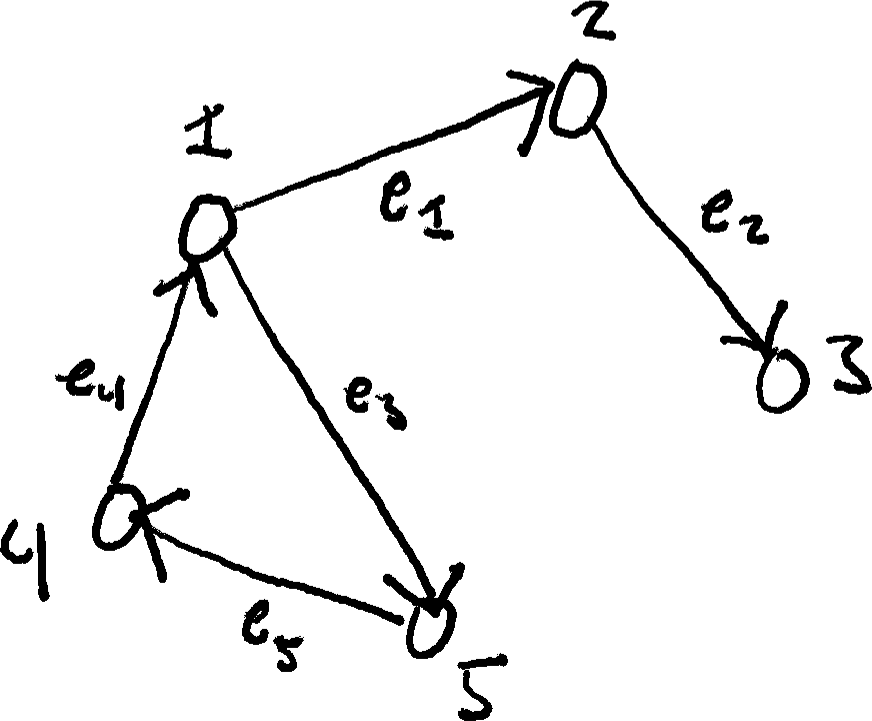
\includegraphics[width=0.5\textwidth]{graphics/L4_spectral/digraph_for_incmat.png}
    \caption{A way of directing the edges of the graph in Figure \ref{fig:graph_for_adjmat}. We have also labelled the edges with their numbers.}
    \label{fig:digraph_for_incmat}
\end{figure}

\begin{example}
    In Figure \ref{fig:digraph_for_incmat} we see one way of directing the edges of the graph in Figure \ref{fig:graph_for_adjmat} to make it a digraph. This digraph has incidence matrix\sidenote[][]{It is a bit unfortunate that our example graph has exactly one cycle, so it has equally many edges and vertices and the incidence matrix is square -- they are of course not in general square.}
    $$\begin{pmatrix}
        -1 & 0 & -1 & 1 & 0 \\
        1 & -1 & 0 & 0 & 0 \\
        0 & 1 & 0 & 0 & 0 \\
        0 & 0 & 0 & -1 & 1 \\
        0 & 0 & 1 & 0 & -1 
        \end{pmatrix}$$
    and so this matrix is also an incidence matrix for our original simple graph.
\end{example}

Having given these definitions, let us start seeing why these matrices are interesting.

\begin{lemma}\label{lemma:ranks_of_incidence_matrix}
    Let $G$ be a finite simple graph on $n$ vertices with $c$ connected components, and $D$ be an incidence matrix of $G$. It holds that
    $$\rank D = n - c.$$

    \begin{proof}
        To begin with, let us see that $\rank D \leq n - 1$. The column sums of $D$ are all zero, since each column contains exactly one $1$ and one $-1$, for the source and target of its associated edge. Therefore, if we take the sum of all the \emph{row}-vectors, each entry will be zero, so we have a non-trivial linear combination of $0$, and hence $\rank D \leq n - 1$.

        Now, assume $G$ is in fact connected -- then, we will show that this linear combination of $0$ is in fact, up to scaling, the only non-trivial linear combination of $0$ with the row-vectors. So, let $r_i$ for $i = 1,\ldots,n$ denote the row-vectors of $D$, and suppose we have a non-trivial linear combination
        $$\sum_{i=1}^n \alpha_i r_i = 0.$$

        Consider a row $k$ for which $\alpha_k \neq 0$ -- in this row, there is a non-zero entry in every column corresponding to an edge incident to the vertex $k$. Each of these columns has one other non-zero entry, and that entry has the opposite sign of the one in our row. So for these to sum to zero, the coefficients in the linear combination must be the same. So what we have seen is that $\alpha_\ell = \alpha_k$ whenever $\ell$ is adjacent to $k$.

        However, we assumed $G$ is connected, so this argument in fact extends to showing that all the coefficients must equal $\alpha_k$, and so this shows the linear combination is indeed just a rescaling of the sum of all the rows.

        Finally, assume $G$ has $c$ connected components, and observe that we can always relabel the vertices and edges in such a way that $D$ is in block-diagonal form, with every block being the incidence matrix of a connected component. So the claim follows from the statement for connected graphs.
    \end{proof}
\end{lemma}

The statement we are looking towards, counting spanning trees, will involve determinants, so let's start proving things about determinants of these matrices.

\begin{lemma}
    Any square submatrix of an incidence matrix $D$ has determinant $0$, $1$, or $-1$.

    \begin{proof}
        We prove this by induction in the size $k$ of the $k\times k$ submatrix. The statement is obvious for $k=1$, since all the entries of an incidence matrix are zero, one, or minus one.

        Now consider a submatrix $M$ of size $(k+1)\times(k+1)$. If every column of $M$ has either two or no non-zero entries, then $\det M = 0$, since then every column will sum to zero. Otherwise, there is a column of $M$ having exactly one non-zero entry. Expanding $m$ along this column yields $\det M = \pm \det M'$ where $M'$ is a $k \times k$ submatrix of $D$. Hence the result follows by induction.
    \end{proof}
\end{lemma}

Now, consider what happens if we pick some set of edges $S \subset E$, and let $D_S$ be just the columns of the incidence matrix that correspond to these edges -- this will in fact be the incidence matrix of the spanning subgraph $(V, S)$ of $G$. So if we pick $S$ as a set of $n-1$ edges, this spanning subgraph will be a spanning tree exactly if it is connected\sidenote[][]{
    \begin{xca}
        Prove that a graph on $n$ vertices and $n-1$ edges is a tree if and only if it is connected.
    \end{xca}
} -- and Lemma \ref{lemma:ranks_of_incidence_matrix} gives us a nice way of checking if it is connected or not: It is connected whenever $\rank D_S = n - 1$.

\begin{lemma}
    Let $S$ be an $n-1$-element subset of the edges of $G$, and let $M$ denote any $(n-1)\times (n-1)$ submatrix of the $n \times (n-1)$ matrix $D_S$. Then $M$ is invertible if and only if $(V,S)$ is a spanning tree of $G$.

    \begin{proof}
        We already observed that $D_S$ has rank $n-1$ whenever $(V,S)$ is a spanning tree, so removing any row from it will create a non-singular square matrix $M$.

        In the other direction, if $M$ is nonsingular, then $D_S$ contains at least $n-1$ linearly independent rows and the same number of linearly independent columns. Hence $\rank D_S = n - 1$ and so $(V,S)$ must be connected and thus a tree.
    \end{proof}
\end{lemma}

\section{Exercises}

%\bibliography{references}
%\bibliographystyle{plainnat}

\end{document}
